\documentclass{rubeamer}
\svnid{$Id: FinalPresentation.tex 2719 2015-11-05 12:57:01Z kristofert13 $}
\svnidlong{$HeadURL: https://repository.cs.ru.is/svn/t-411-mech-2015/group/TiltIt/FinalPresentation/FinalPresentation.tex $}
{$LastChangedDate: 2015-11-05 12:57:01 +0000 (fim., 05 nóv. 2015) $}
{$LastChangedRevision: 2719 $}
{$LastChangedBy: kristofert13 $}
% if you'd like the above information to be updated,
% use svn properties to set svn:keywords to for Id and URL (or HeadURL)
% Don't forget to set the draft to final before 

\addbibresource{references.bib}


\begin{document}
%----------- titlepage ----------------------------------------------%
\rutitleframe{}

%----------- slides ----------------------------------------------%

\begin{frame}{Introduction}
	\begin{itemize}
		\item Above all the project has to be challenging and interesting!
		\item Doesn't necessarily have to solve pre-existing problems.
	\end{itemize}
	\note{The basic idea and its complications. Have a separate slide for the gif?}
\end{frame}

\begin{frame}{The Stewart Platform}
	\begin{figure}
		\centering
		\animategraphics[loop,autoplay,scale=0.7]{12}{gifs/hex-}{1}{23}
		\caption*{GIF a user made for Wikipedia~\cite{gif_hex}}
	\end{figure}
\end{frame}

\begin{frame}{How can you use this?}
	\vspace{1em}
	\begin{itemize}
		\item AR Games/Simulations
		\item Stabilizing equipment
		\item Fun
	\end{itemize}
	
	\begin{figure}
		\centering
		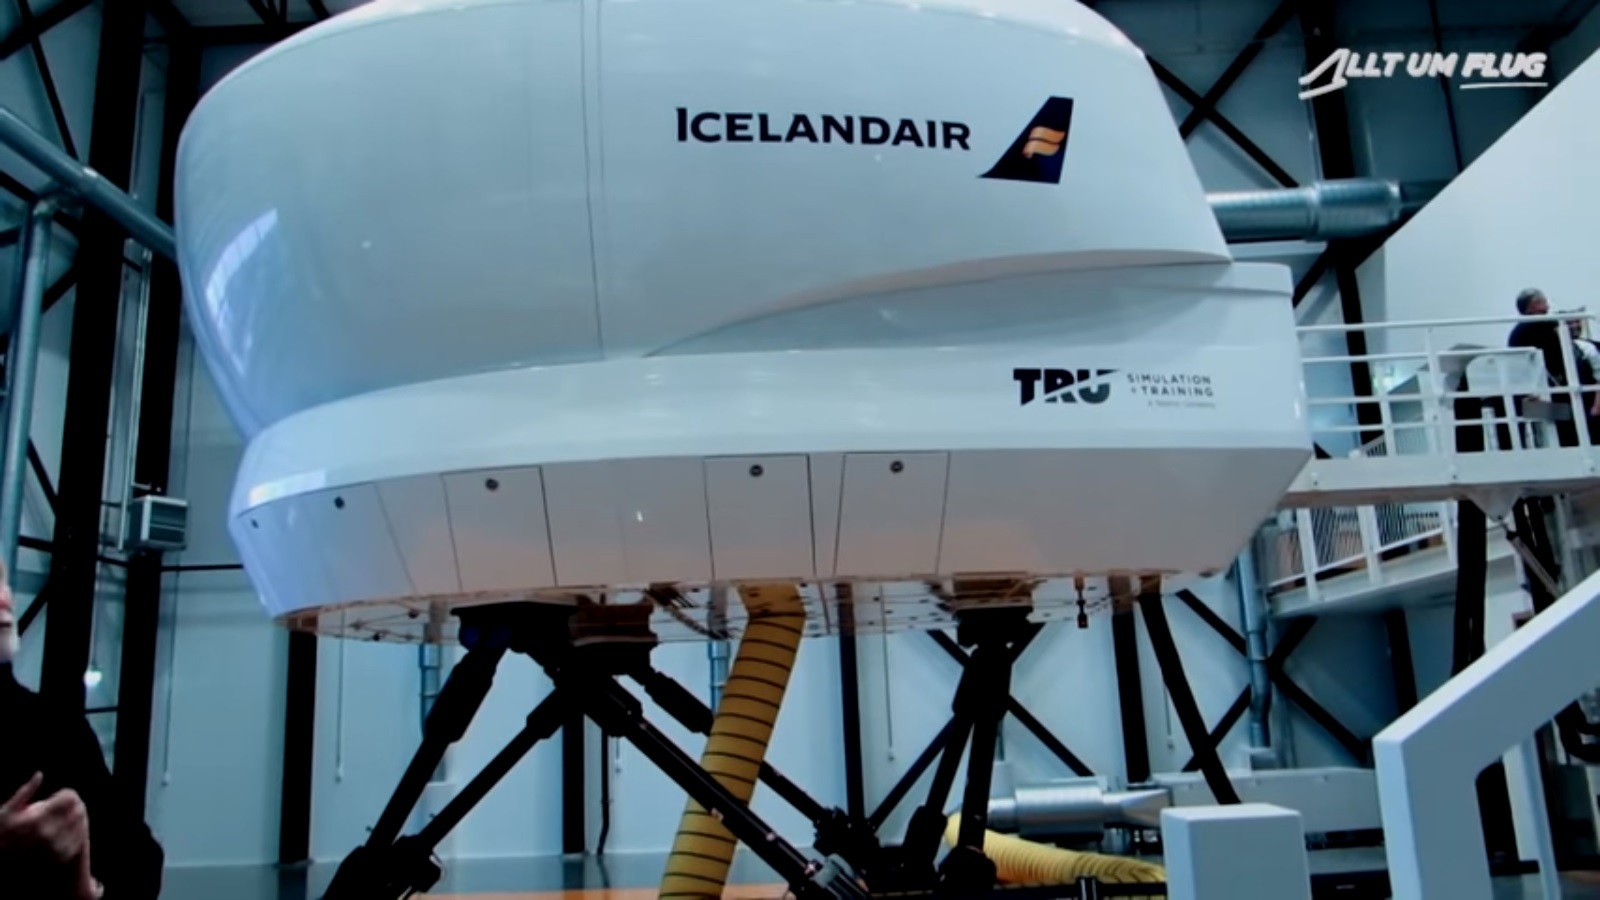
\includegraphics[scale=0.18]{icelandair}
		\caption*{Flight sim in use by Icelandair~\cite{icelandair}}
	\end{figure}
\end{frame}

\begin{frame}
	\begin{figure}
		\centering
		
\includegraphics[page=4, scale=0.42]{NASAdocking.pdf}
		\caption*{NASA's Low-impact docking system \cite{pres:NASAdock}}
	\end{figure}
\end{frame}

\begin{frame}{What is a good solution?}
	\begin{itemize}
		\item Requires a good design!
		\item Smooth movements while maintaining speed
		\item Has to be accurate
	\end{itemize}
\end{frame}

\begin{frame}{Where we got the design}
	\begin{itemize}
		\vspace{1em}
		\item Frame design~\cite{sp}
		\item RUMBA firmware~\cite{sp_code}
	\end{itemize}
	
	\begin{figure}
		\subfloat{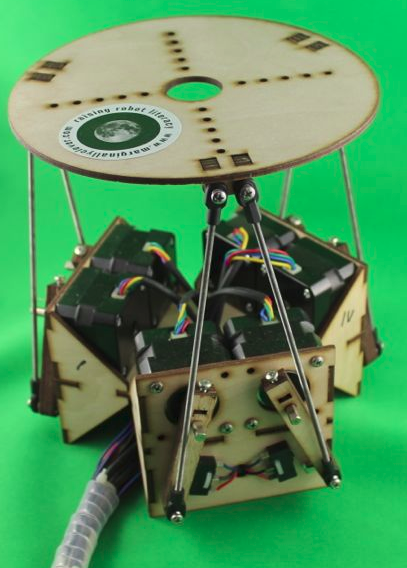
\includegraphics[scale=0.24]{graphics/sp_pic.png}}~
		\subfloat{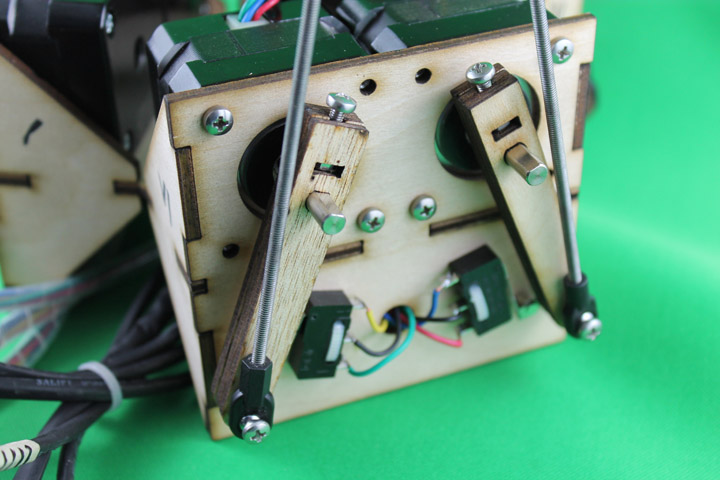
\includegraphics[scale=0.28]{sp_design_arms}}
		\caption*{Figures from MarginallyClever~\cite{sp}}
	\end{figure}	
\end{frame}

\begin{frame}{Problems encountered}
	\vspace{3em}
	\begin{itemize}
		\item Connecting the motors and switches correctly to the RUMBA
		\item Communications: Controller $\rightarrow$ Arduino $\rightarrow$ RUMBA
		\item Wiring from controller to Arduino
		\item \textit{Getting the platform to tilt\\correctly}
	\end{itemize}
	
	\begin{figure}
		\vspace{-3em}
		\raggedleft
		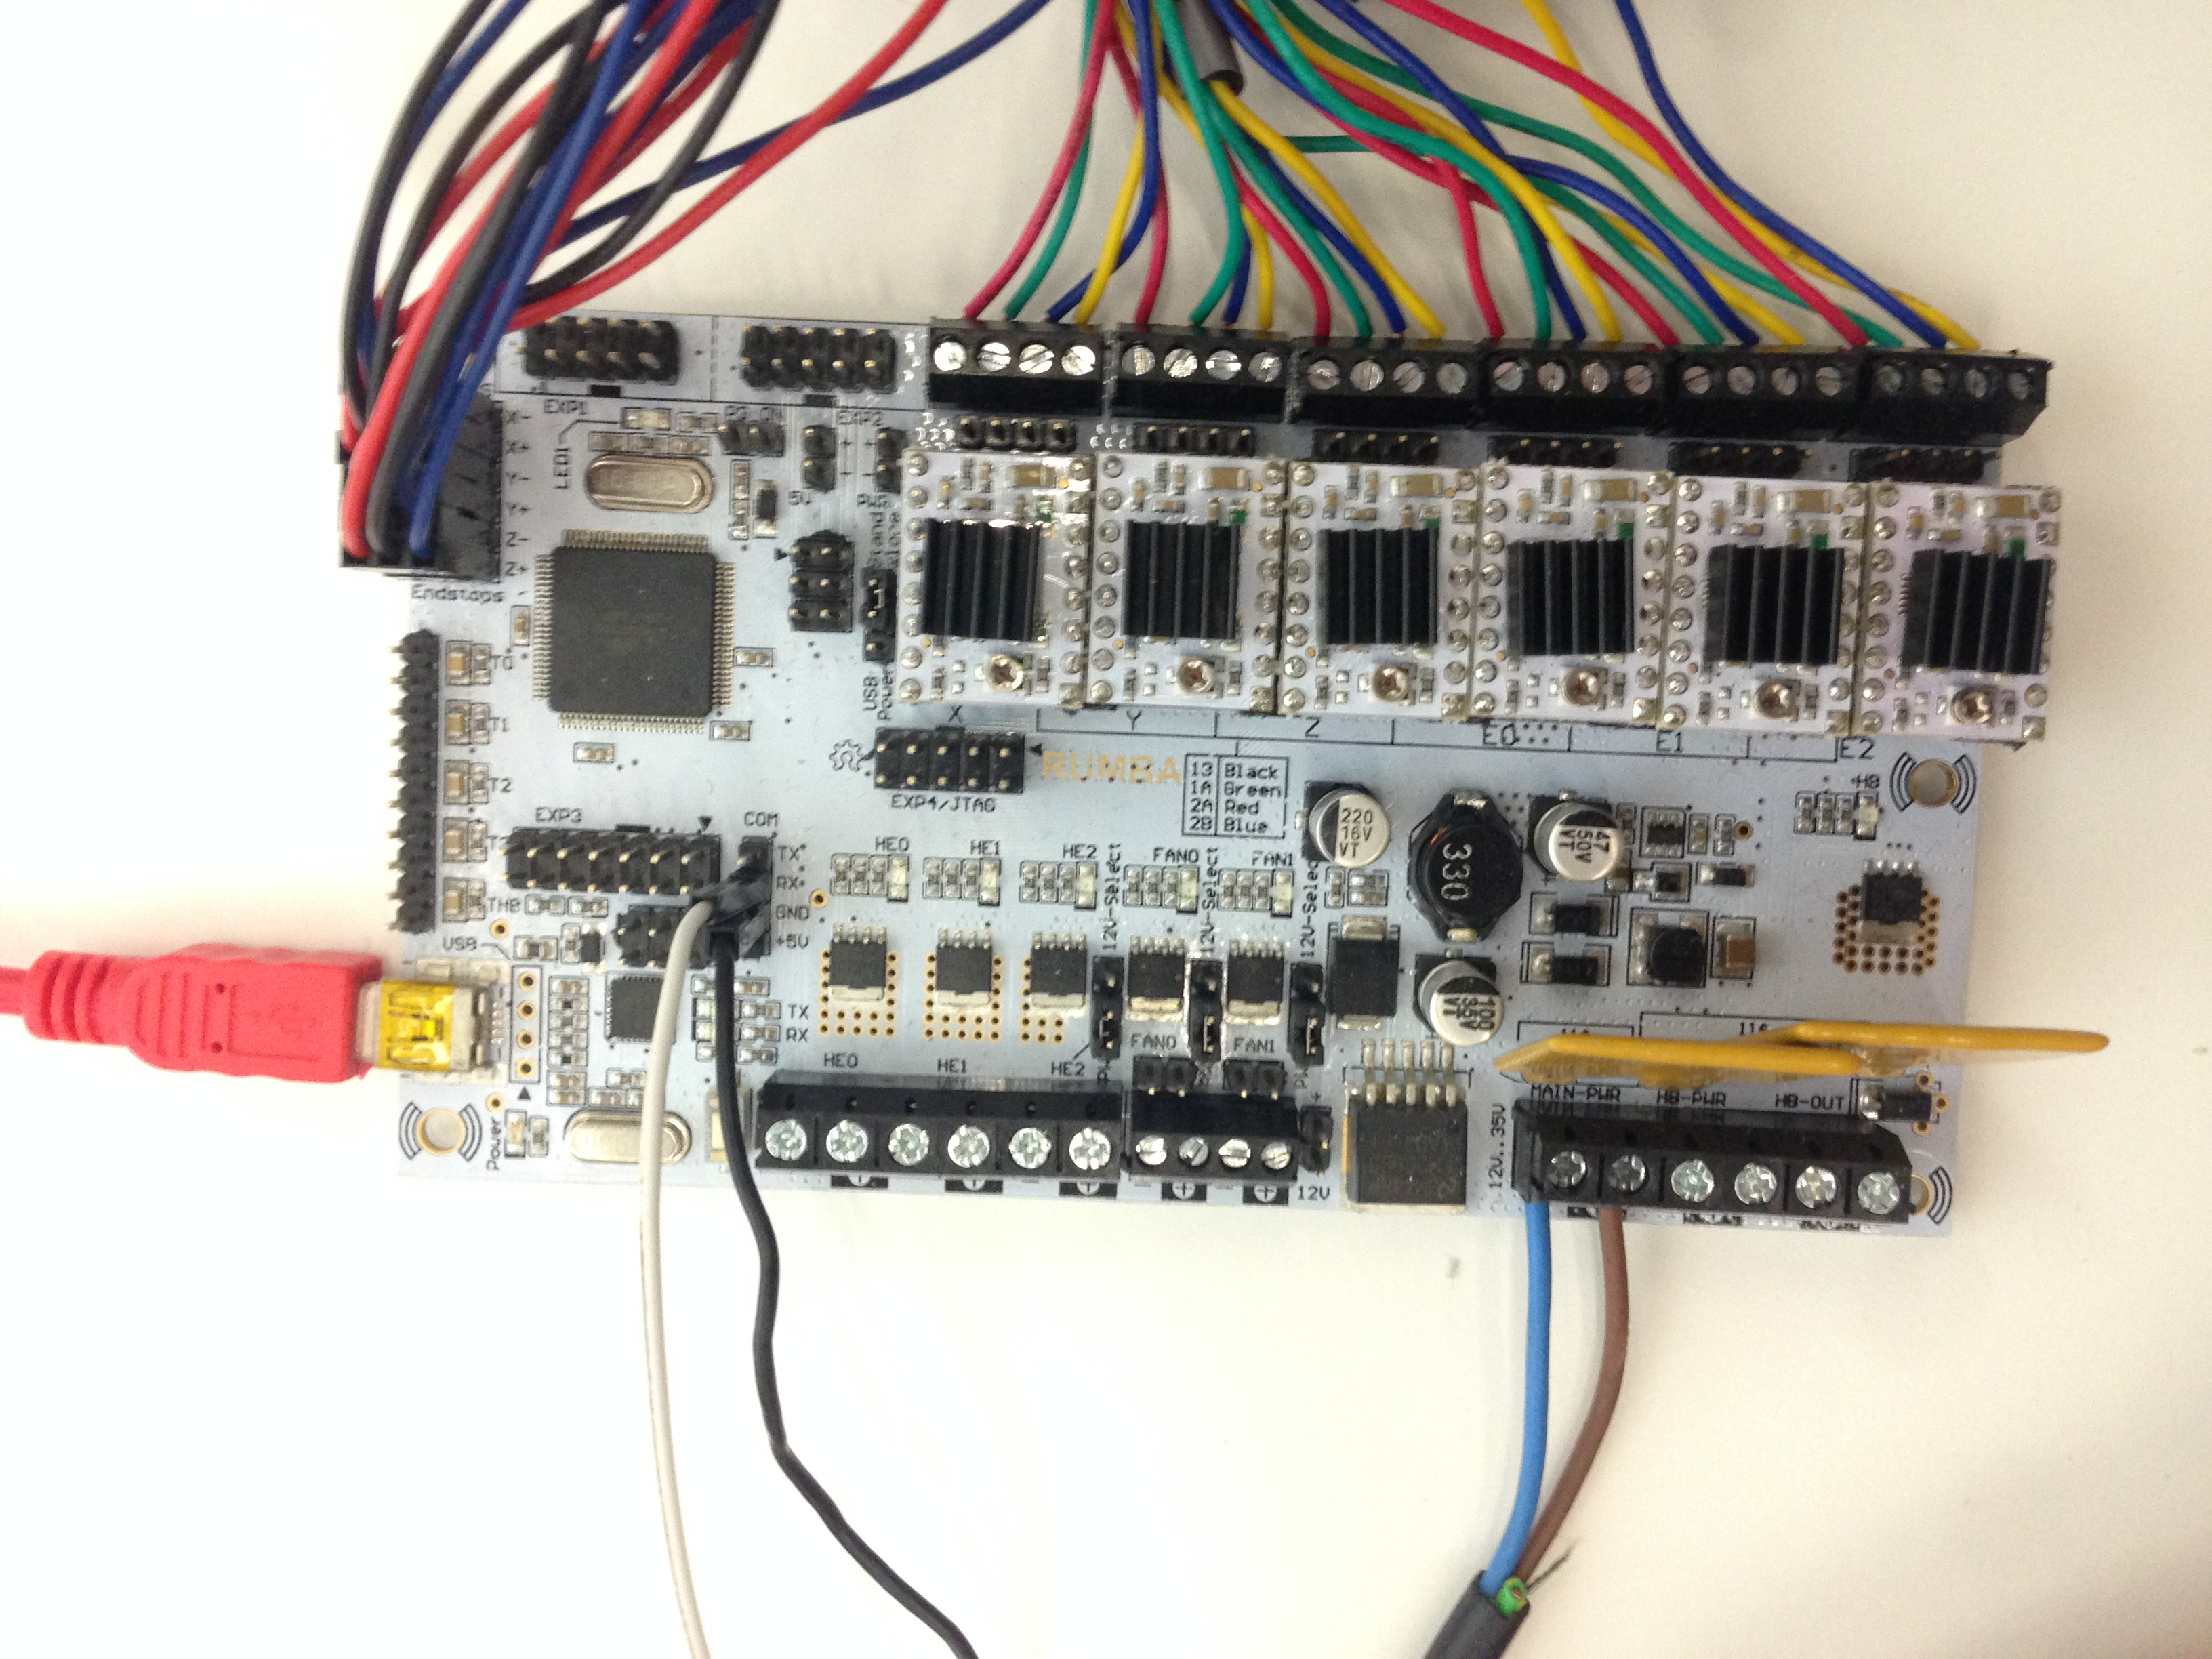
\includegraphics[scale=0.05]{rumba}
		\caption*{\hspace{20em}The RUMBA motor controller}
	\end{figure}
\end{frame}

\begin{frame}{Operation flowchart}
	\begin{center}
		\begin{tikzpicture}
		\node(contr)[startstop]{Controller};
		\node(ard)[process, below of=contr, yshift = -0.7cm]{Arduino};
		\node(rumba)[process, below of=ard, yshift = -0.7cm]{RUMBA};
		\node(motors)[startstop, below of=rumba, yshift = -0.7cm]{Motors};
		
		\draw[arrow](contr)--node[anchor=west]{input}(ard);
		\draw[arrow](ard)--node[anchor=west]{command}(rumba);
		\draw[arrow](rumba)--node[anchor=west]{movement}(motors);
		\end{tikzpicture}
	\end{center}
	\note{What's the best place for this slide?}
\end{frame}

\begin{frame}{Price}
	\begin{itemize}
		\item 8 x Stepper motors
		\begin{itemize}
			\item Model: ROB-09238 from Sparkfun\cite{sf_motor}
			\item 2350 ISK per unit
		\end{itemize}
	\end{itemize}
	\begin{itemize}
		\item RUMBA Motion Controller
		\begin{itemize}
			\item Model: ELEC-0038 from MarginallyClever \cite{sp}
			\item 29950 ISK
		\end{itemize}
	\end{itemize}
	\begin{itemize}
		\item Custom made cables
		\begin{itemize}
			\item Smith \& Norland ehf. donated two custom cables
		\end{itemize}
	\end{itemize}
	\begin{itemize}
		\item Plexi-glass
		\begin{itemize}
			\item Fást donated the plexi-glass
		\end{itemize}
	\end{itemize}
	\bigskip
	\textbf{Total price: $\mathbf{\sim}$70.000 ISK}
\end{frame}

\begin{frame}{Assembly}
	\begin{figure}
		\centering
		\subfloat{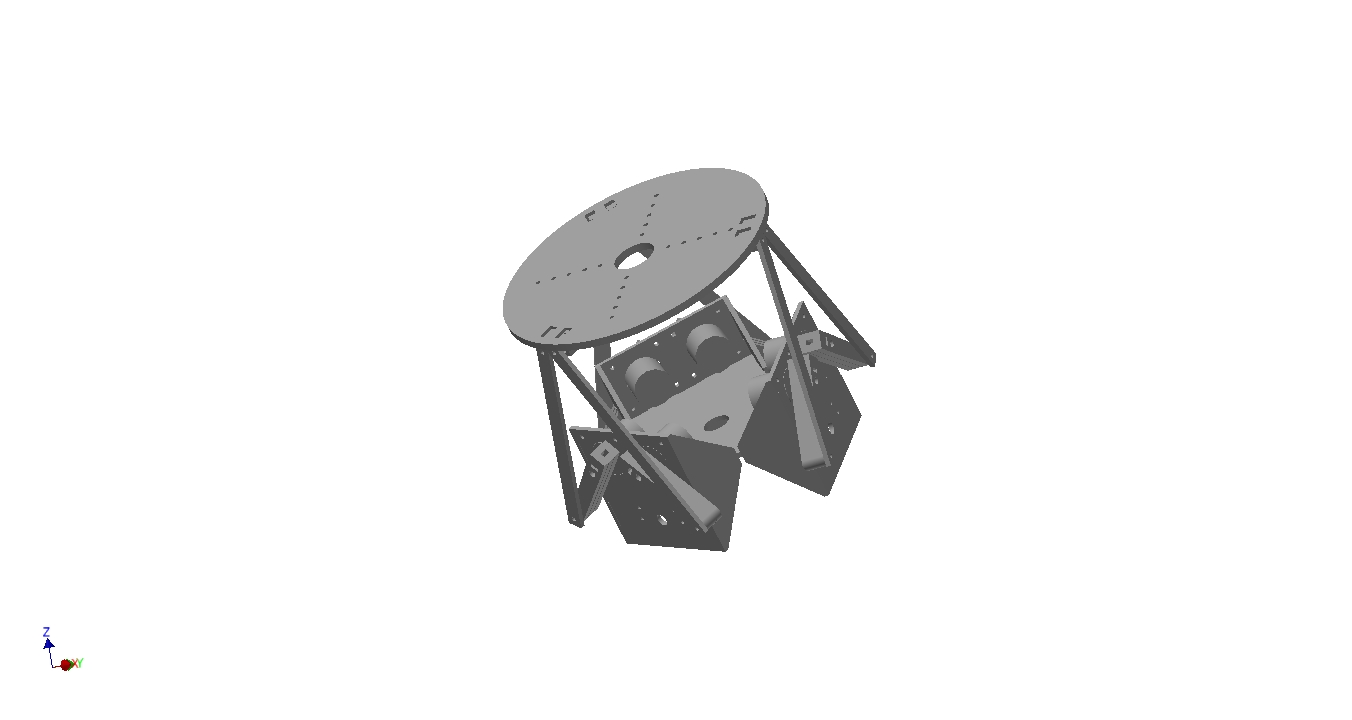
\includegraphics[scale=0.5,trim={13cm 4.5cm 12cm 4cm},clip]{stewy}}
		\subfloat{\includegraphics[scale=0.15]{../FinalReport/graphics/controller_4pics}}
		\caption*{CAD designs}
	\end{figure}
\end{frame}

\begin{frame}{Assembly}
	\begin{figure}
		\centering
		\subfloat{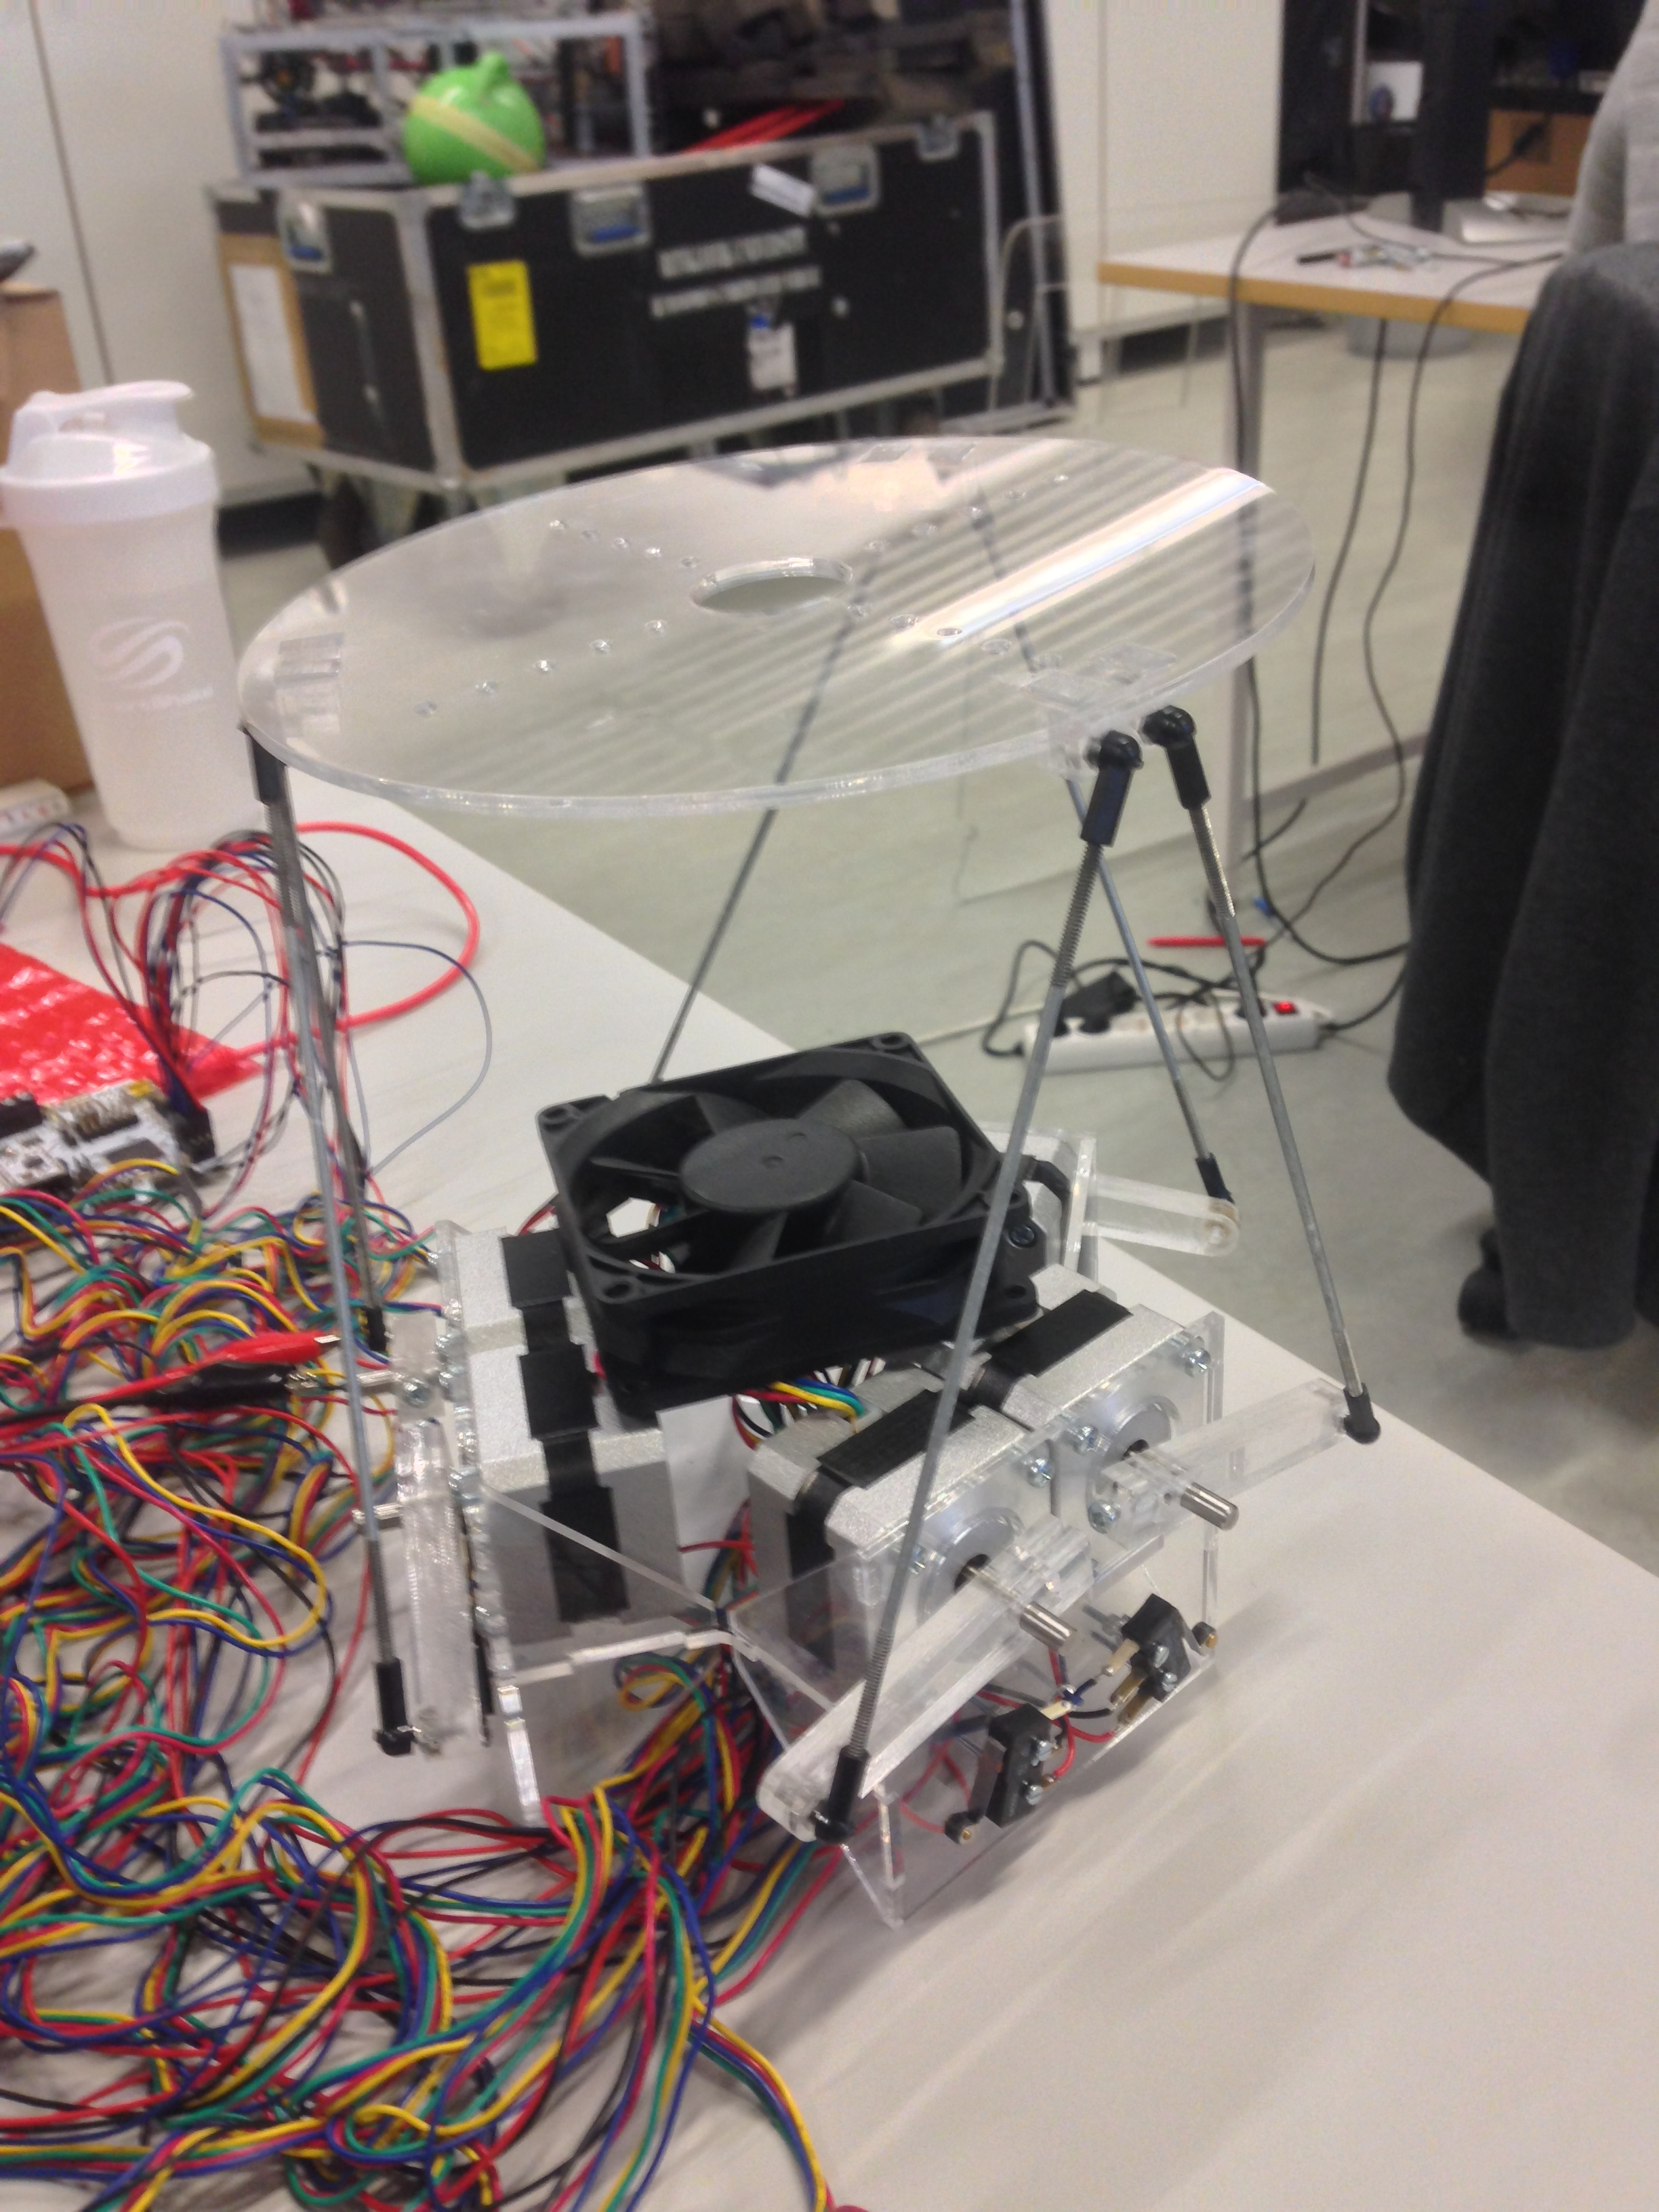
\includegraphics[scale=0.057]{platform_testing}}~
		\subfloat{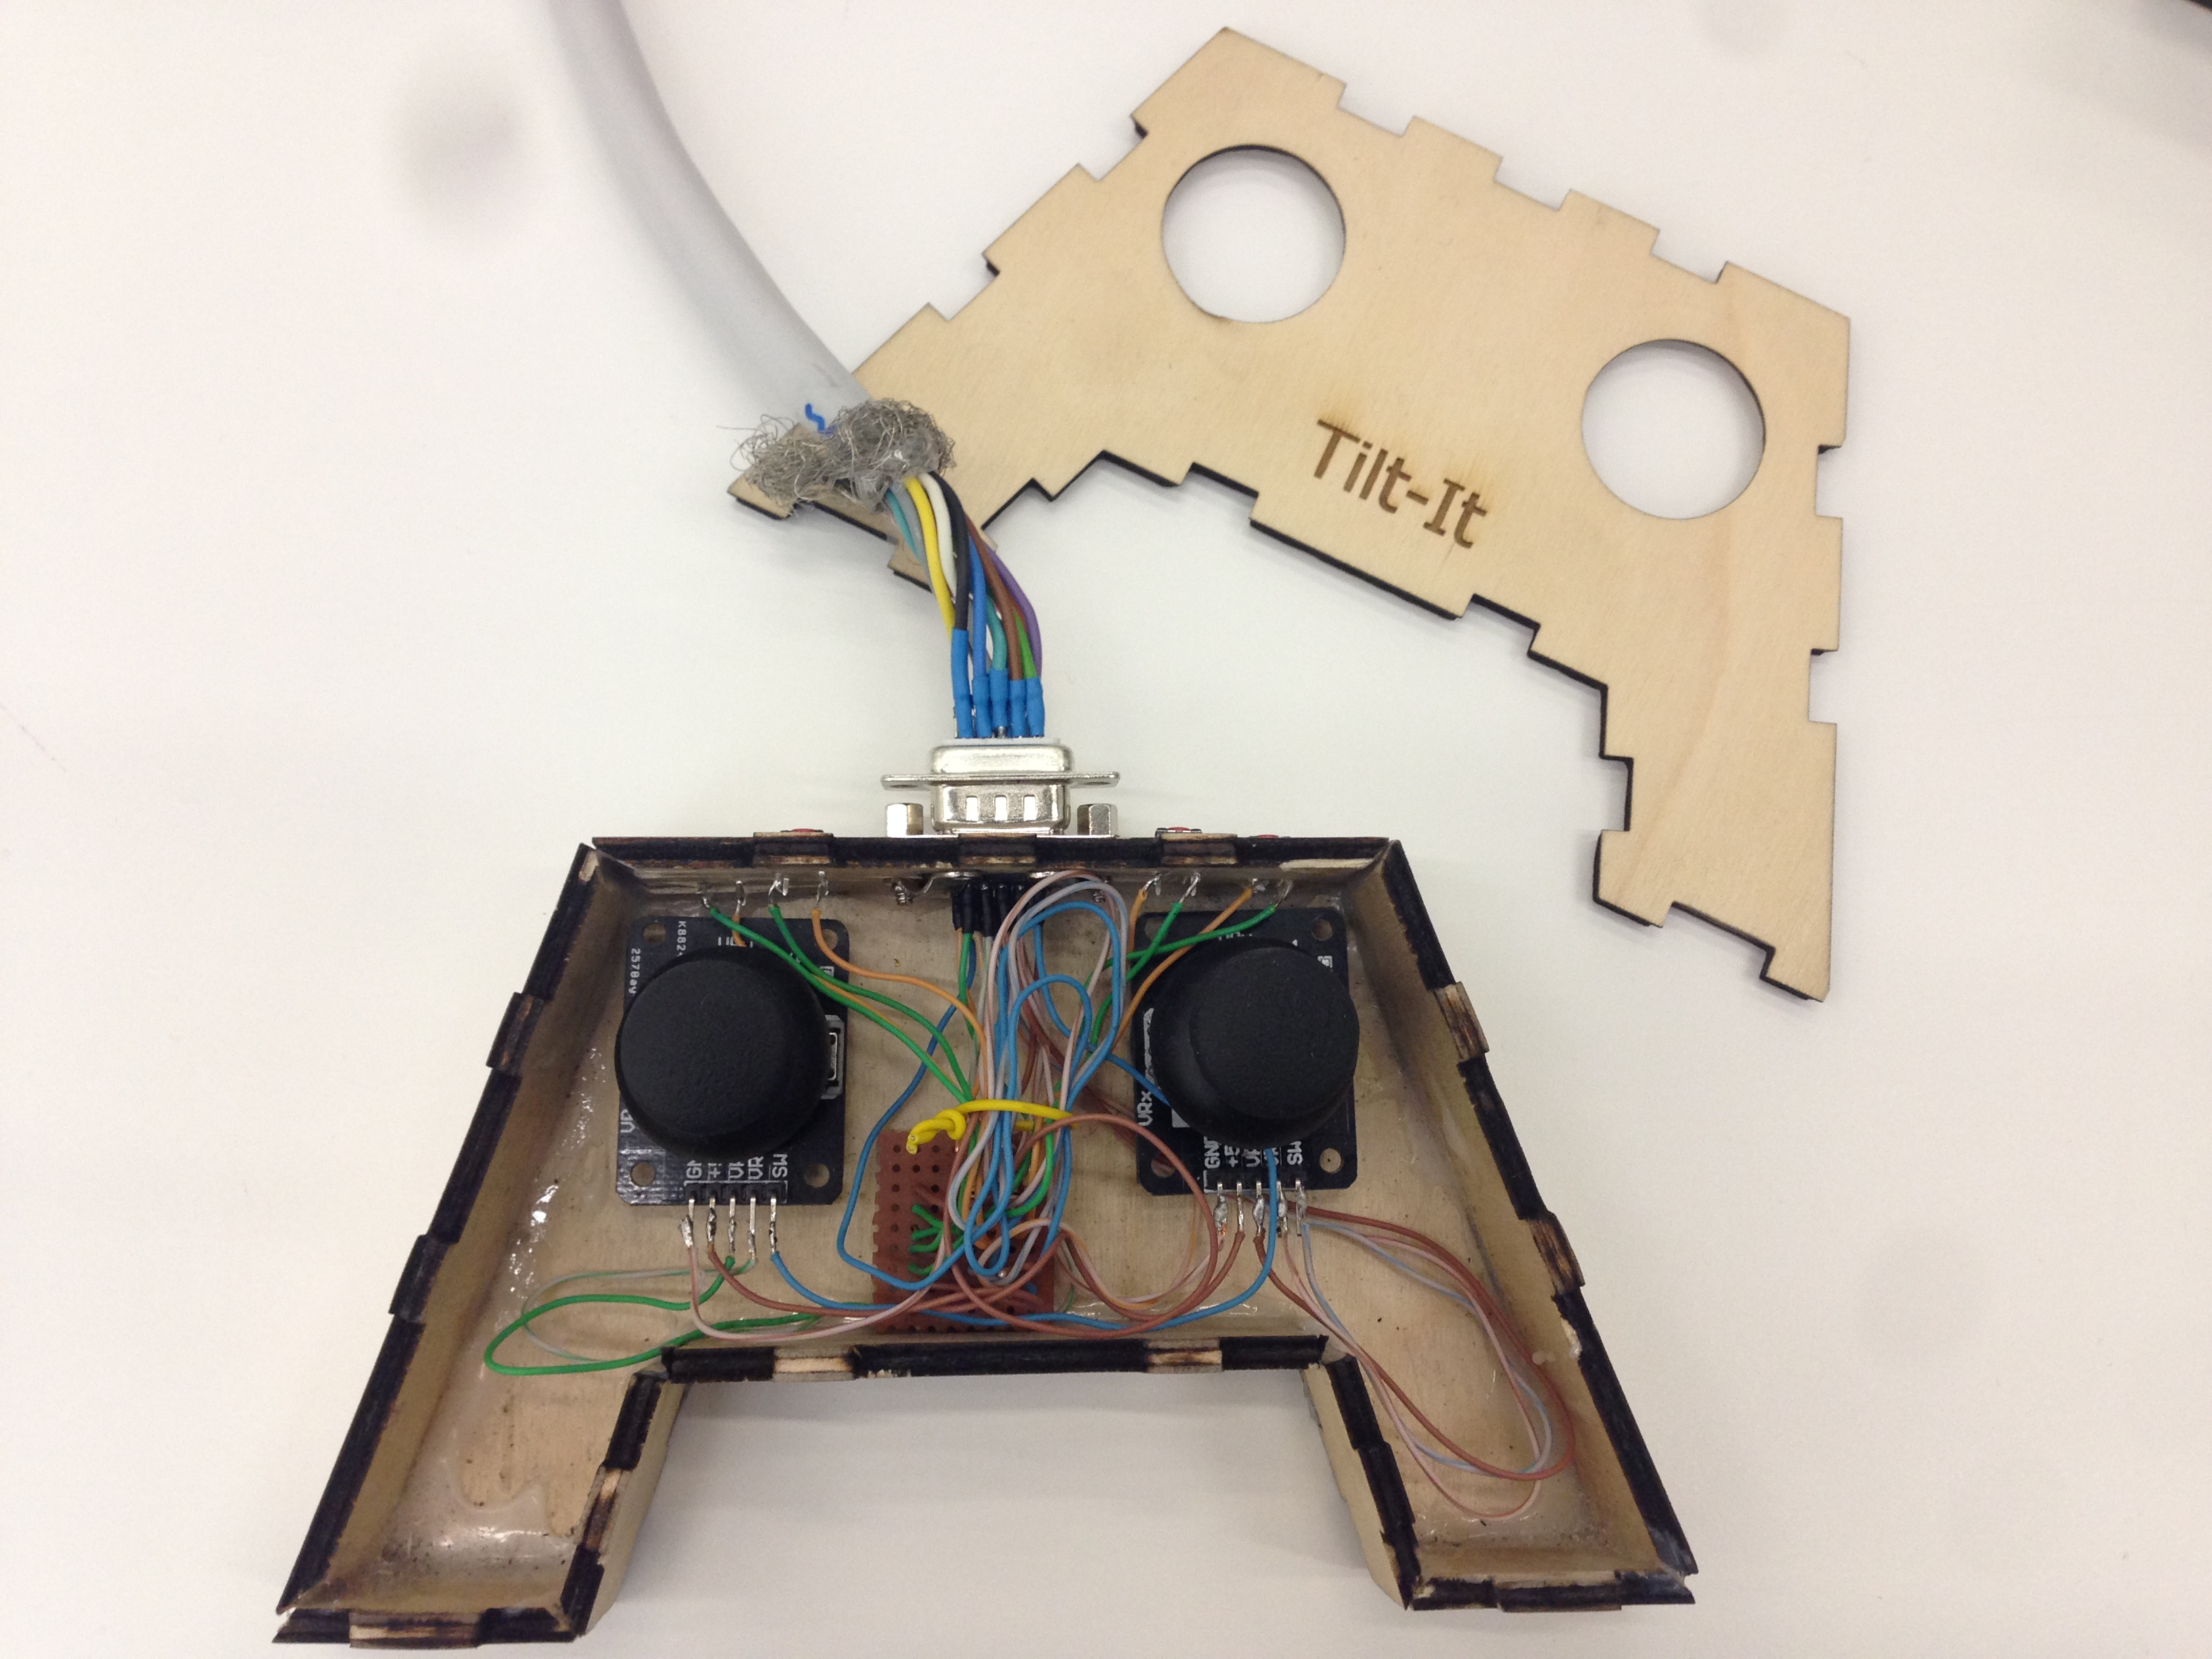
\includegraphics[scale=0.057]{contr_open_3}}
		\caption*{During testing}
	\end{figure}
\end{frame}

\begin{frame}{Results}
	\begin{figure}
		\centering
		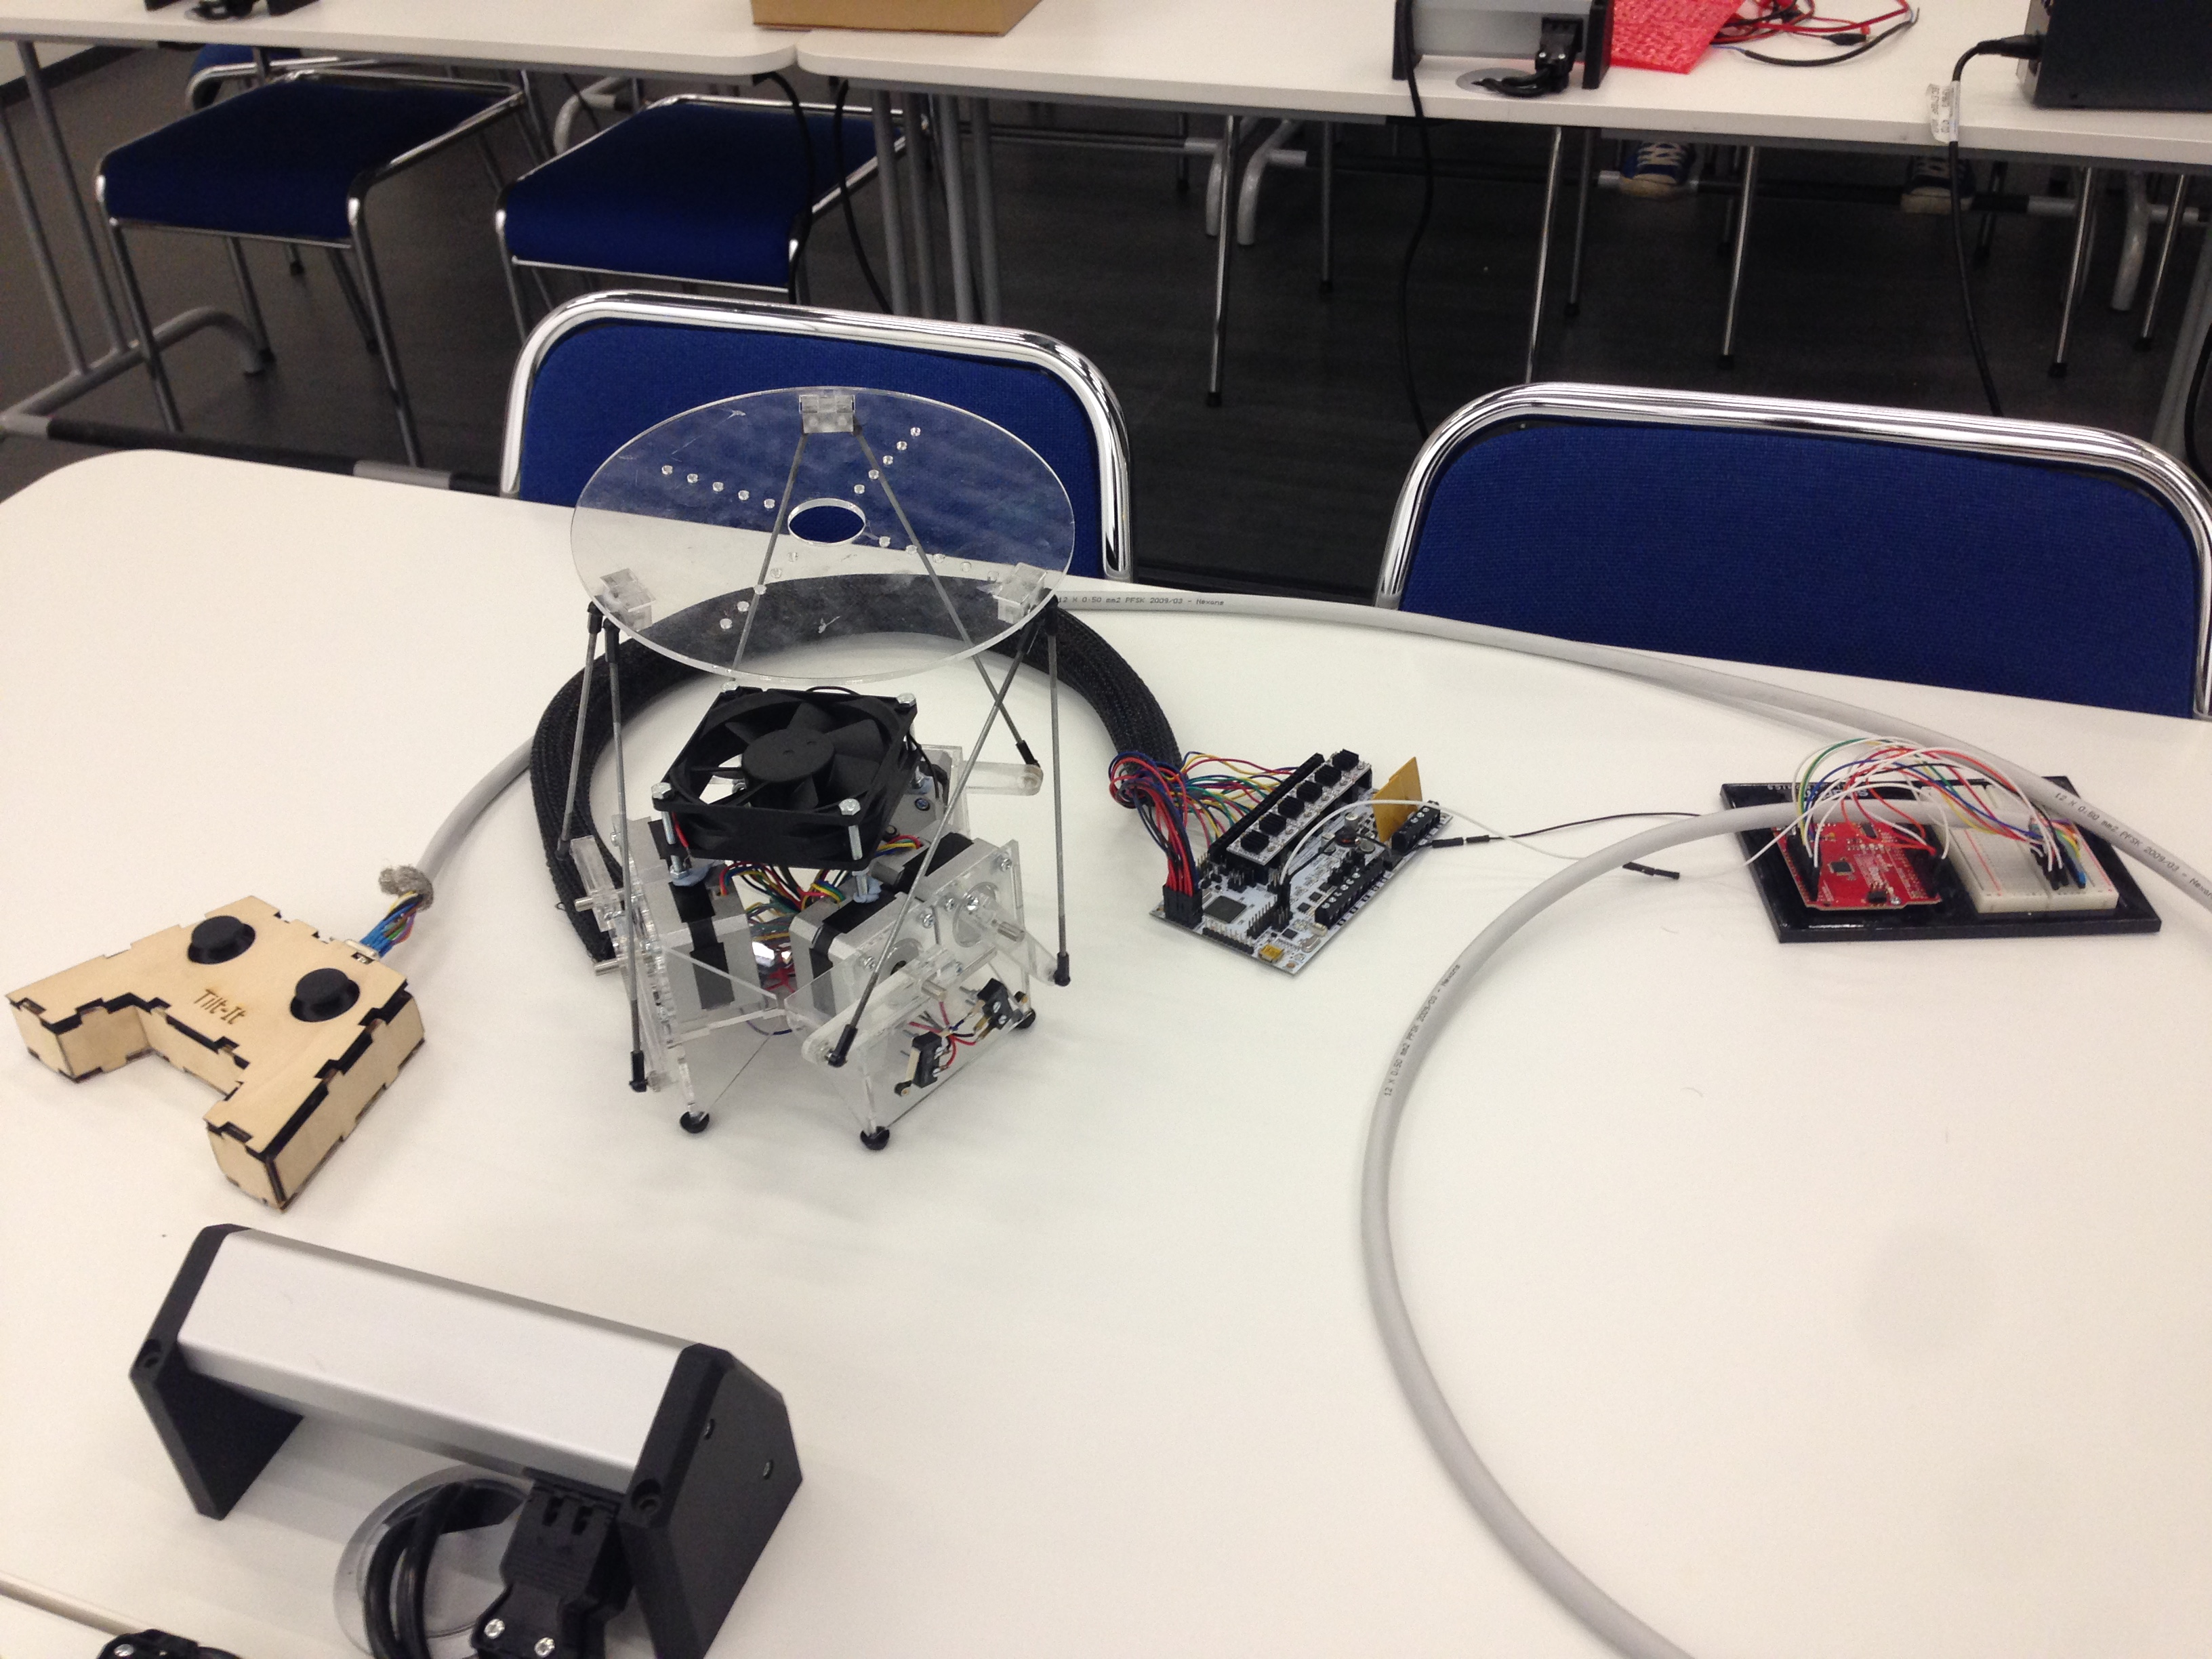
\includegraphics[scale=0.1, trim=0em 45em 0em 40em, clip]{platform_final}
		\caption*{End result}
	\end{figure}
\end{frame}

\begin{frame}{Unresolved issues}
	\begin{itemize}
		\item Smoothness when moving
		\item Proper sensitivity
	\end{itemize}
\end{frame}

\begin{frame}{Future ideas}
	\vspace{3em}
	\begin{itemize}
		\item Wireless controller
		\item Game platform - e.g. Maze Game
		\item Make it bigger
	\end{itemize}
	
	\begin{figure}
		\vspace{-3em}
		\centering
		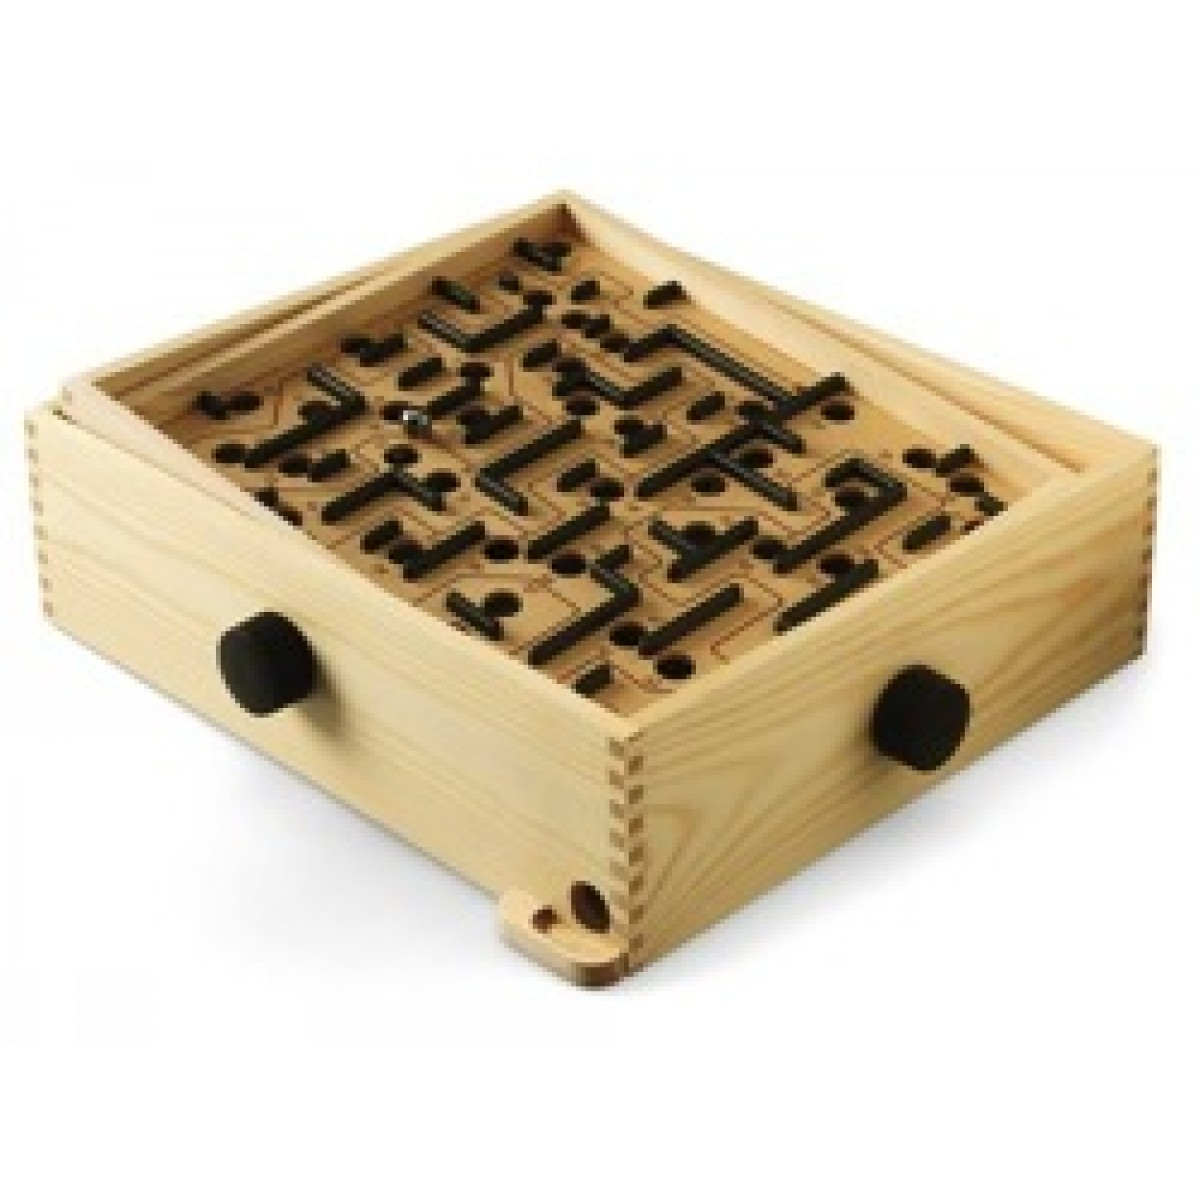
\includegraphics[scale=0.1, trim=0em 20em 0em 0em]{veltipete}
		\caption*{Maze game~\cite{veltipete}}
	\end{figure}
\end{frame}
\begin{frame}
	\centering
	Thank you for your time.
	Questions?\\
\end{frame}

\bibframe
\end{document}

%%% Local Variables:
%%% mode: latex
%%% TeX-master: t
%%% End:
